\documentclass[table, 12pt]{article}
\usepackage[T1]{fontenc}
\usepackage[utf8]{inputenc}
\usepackage[english]{babel}
\usepackage{graphicx}
\usepackage{titlesec}
\usepackage{hyperref}
\usepackage[usenames,dvipsnames]{xcolor}
\usepackage{float}
\usepackage[export]{adjustbox}
\usepackage{longtable}

\hyphenation{Te-lan-ga-na}
\hyphenation{an-a-lys-ing}
\hyphenation{a-gron-o-mists}
\hyphenation{a-gron-o-mist}
\titleformat{\paragraph}
{\normalfont\normalsize\bfseries}{\theparagraph}{1em}{}
\titlespacing*{\paragraph}
{0pt}{3.25ex plus 1ex minus .2ex}{1.5ex plus .2ex}


\begin{document}
\begin{titlepage}
    \centering
    {\scshape\large AY 2021/2022 \par}
    \vfill
    
\includegraphics[width=100pt]{assets/logo-polimi-new}\par\vspace{1cm}
    {\scshape\LARGE Politecnico di Milano \par}
    \vspace{1.5cm}
    {\huge\bfseries DD\@: Design Document \par}
    \vspace{2cm}
    {\Large {Ottavia Belotti\quad Alessio Braccini\quad Riccardo Izzo}\par}
    \vfill
    {\large Professor\par
        Elisabetta \textsc{Di Nitto}}
    \vfill
    {\large \textbf{Version 1.0}\\ \today \par}
\end{titlepage}

\hypersetup{%
    pdfborder = {0 0 0}
}

\thispagestyle{plain}
\pagenumbering{gobble}
\mbox{}
\newpage
\pagenumbering{roman}
\tableofcontents
\newpage
\pagenumbering{arabic}

\section{Introduction}


\subsection{Purpose}
The purpose of this document is to provide a full technical description of the system described in the RASD document.
In this design document we discuss about both hardware and software architectures in terms of interaction among the components that represent the system.
Moreover, there are mentions about the implementation, testing and integration process.
This document will include technical language so it is primarily addressed to programmers, but stakeholders are also invited to read it in order to understand the characteristics of the project.

\subsection{Scope}
The scope of this design document lays in the definition of the system behavior, in both general and critical cases, and in the design of the system architecture by describing the
logical allocation of the components and the interaction between them.
This document also extends in part to the implementation and testing plan, where one possible course of action is explained, user interface design of user applications and requirements traceability relating to the RASD.
\subsection{Definitions, acronyms, abbreviations}
\subsubsection*{Acronyms}
\begin{itemize}
    \item \textbf{DREAM}: \emph{Data-driven predictive farming}
    \item \textbf{RASD}: Requirement Analysis and Specification Document
    \item \textbf{DD}: Design Document
    \item \textbf{API}: Application Programming Interface
    \item \textbf{DBMS}: Database Management System
    \item \textbf{UML}: Unified Modeling Language
    \item \textbf{GPS}: Global Positioning System
    \item \textbf{IT}: Information Technology
    \item \textbf{GUI}: Graphic User Interface
    \item \textbf{UI}: User Interface
\end{itemize}
\subsection{Revision history}

\subsection{Reference documents}
\begin{itemize}
    \item Specification document: "Assignment RDD AY 2021-2022"
    \item Requirements Analysis Specification Document (RASD)
    \item UML documentation: https://www.uml-diagrams.org/
    \item ArchiMate documentation: https://pubs.opengroup.org/architecture/archimate3-doc/
    \item Slides of the lectures
\end{itemize}
\subsection{Document structure}
\begin{itemize}
    \item \textbf{Section 1} gives a brief description of the design document, it describes the purpose and the scope of it including all the definitions, acronyms and abbreviations used. 
    \item \textbf{Section 2} delves deeply into the system architecture by providing a detailed description of the components, the interfaces and all the technical choices made for the development of the application.
    It also includes detailed sequence, component and ArchiMate diagrams that describe the system in depth .
    \item \textbf{Section 3} contains a complete description of the user interface (UI), it includes all the client-side mockups with some graphs useful to understand the correct execution flow.
    \item \textbf{Section 4} links the RASD to the DD, it maps the goals and the requirements described in the RASD to the actual functionalities presented in this DD.
    \item \textbf{Section 5} presents a description of the implementation, testing and integration phases of the system components that are going to be carried out during the technical development of the application.
\end{itemize}
\section{Architectural Design}


\subsection{Overview}
\begin{center}
    \begin{figure}[H]
        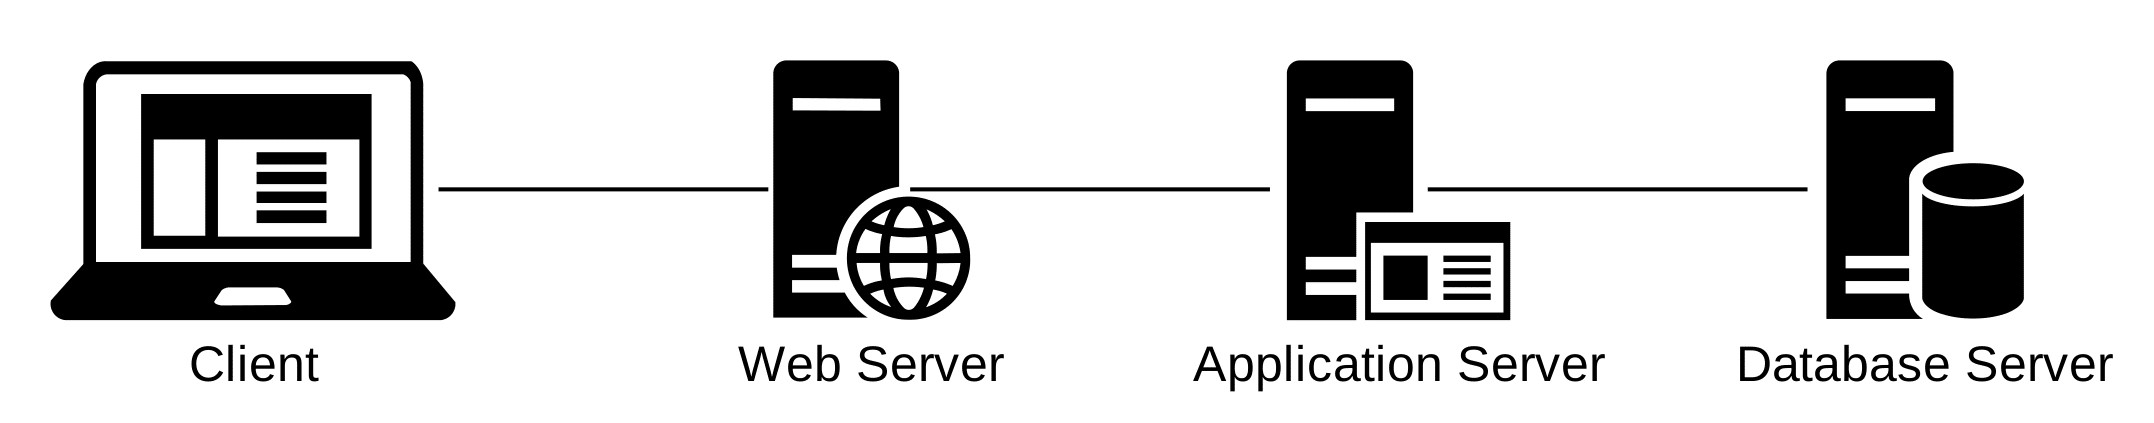
\includegraphics[scale=0.55, center]{assets/4-tier-scheme.jpg}
        \caption{Four-Tier Architecture Scheme}
        \label{fig: four-tier-architecture-scheme}
    \end{figure}
\end{center}

The system is a distributed application that follows the common client-server paradigm.
The architecture of the application is structured in three logic layers:
\begin{itemize}
    \item \textbf{Presentation Layer (P)}: it manages the presentation logic and handles the user actions.
    It is characterized by a GUI (Graphic User Interface) that allows the user to interact with the application in a simple and effective way.
    \item \textbf{Logic or Application Layer (A)}: it manages all the functionalities that has to be provided to the users, it is also responsible of data exchange between the client and the data sources.
    \item \textbf{Data Layer (D)}: it manages the access to data sources, it gets data from the database and moves it through the other layers.
    It is essential to guarantee a high level of abstraction from the database in order to provide an easy to use model.
\end{itemize}

\begin{center}
    \begin{figure}[H]
        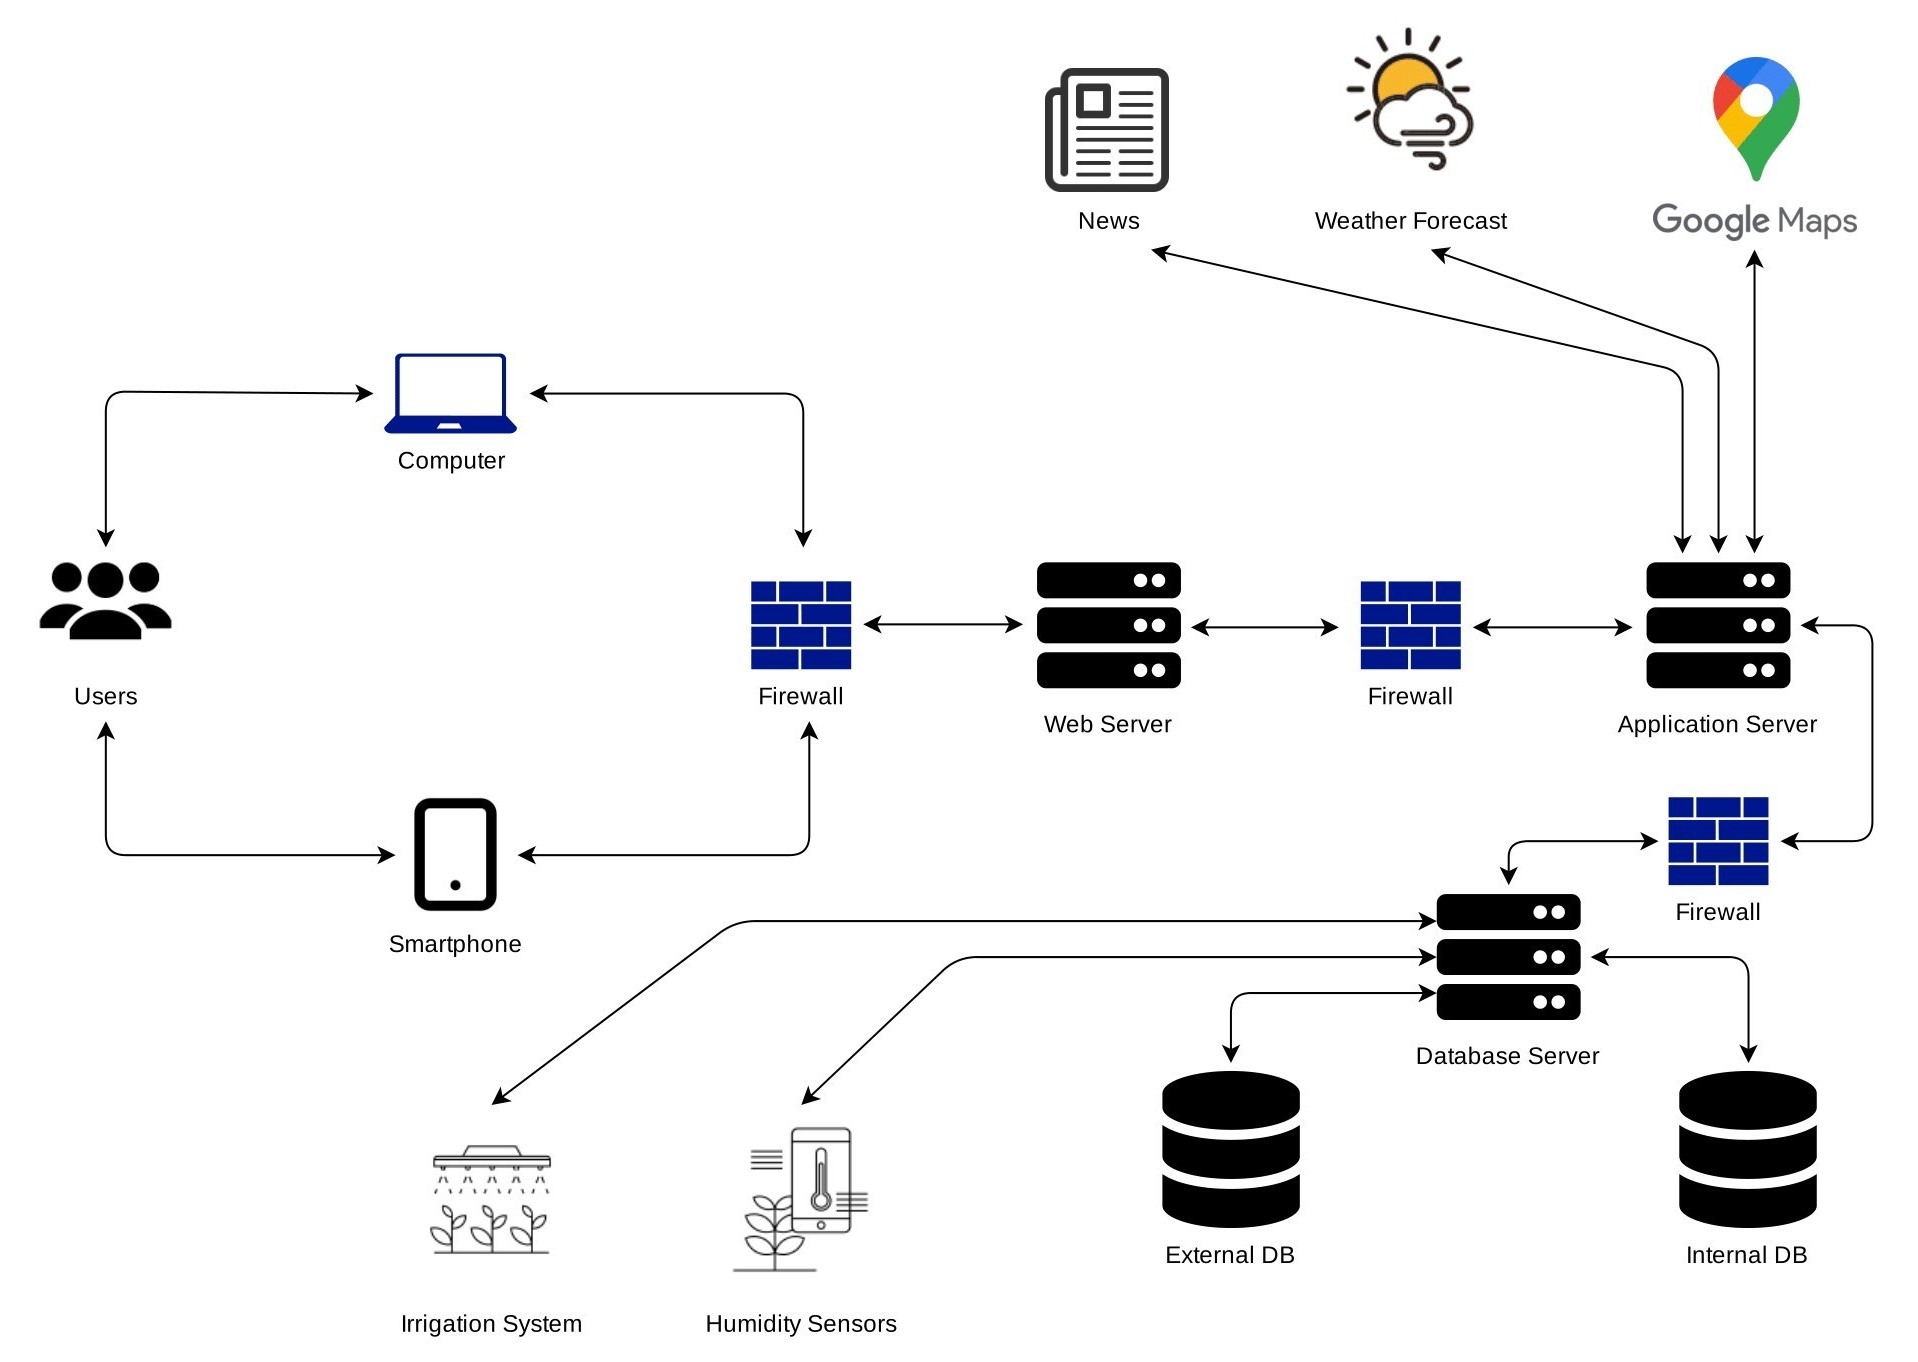
\includegraphics[scale=0.70, center]{assets/4-tier-architecture-scheme.jpg}
        \caption{High Level Architecture}
        \label{fig: high_level_architecture}
    \end{figure}
\end{center}

The system, as shown in \textit{Figure (\ref{fig: four-tier-architecture-scheme})}, is based on a four-tier architecture (Client, Web Server, Application Server and Database Server), this ensures more flexibility and high scalability.
The tiers are separated by firewalls in order to guarantee a higher level of security to the whole system.
A thin client is used to prevent heavy computation load client side, in this way all the heavy operations are executed at server side.
The client's devices can be a personal computer, a mobile device or any kind of IT device able to connect to the Web Server through a web browser. In fact, the four-tiers architecture has been specifically chosen to allow the widest variety of commercial devices to access the application, without the need of developing an OS-specific one for each of them.

The Application Server communicates with the Database Server and transform data following its business logic.
It also manages the news and the weather forecast services.
This allows to retrieve data like weather information directly from it in order to show them to the user.
Finally, to enable the geolocalization, the Application Server uses the API provided by Google Maps.
For what concern the other components, such as the water irrigation system and the humidity sensors, they are connected to the Database Server that exchanges data with the Application Server.
%The Web Server also manages the data coming from the irrigation system and the humidity sensors.
All the components will be described in depth in the following sections.

\subsection{Component view}
\subsubsection*{General Component View}
\begin{center}
    \begin{figure}[H]
        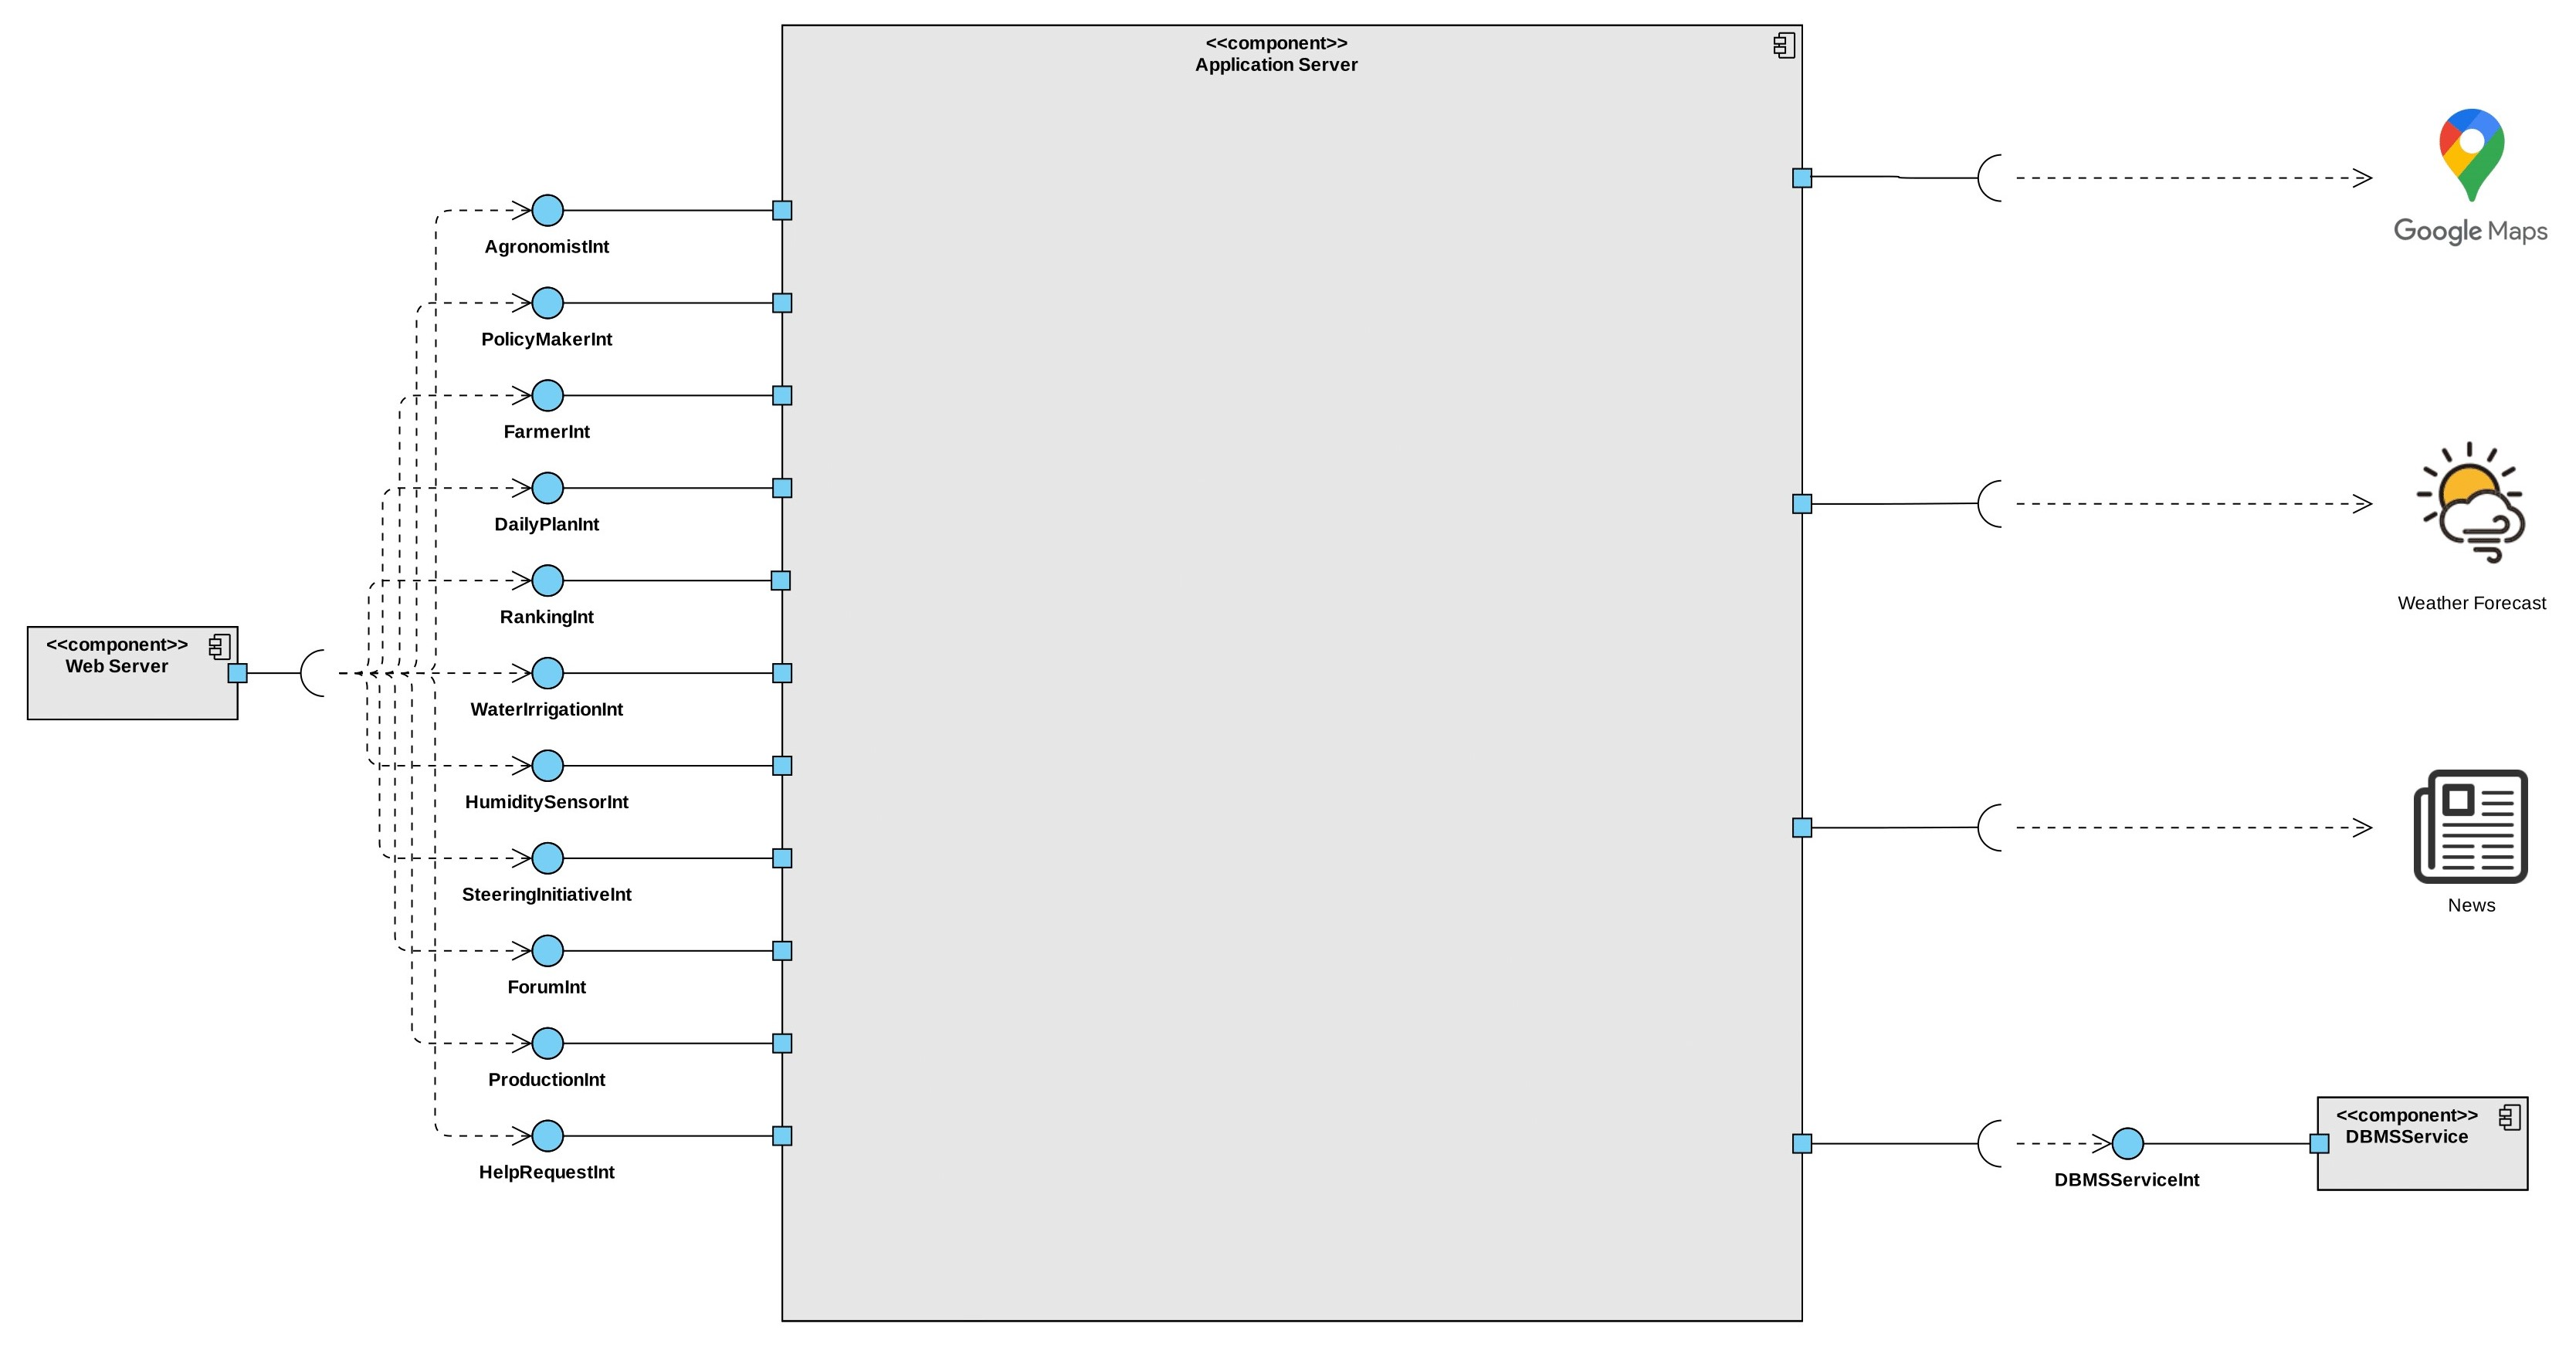
\includegraphics[scale=0.50, center]{assets/general-component-view.jpg}
        \caption{General Component Diagram}
        \label{fig: general_component_view}
    \end{figure}
\end{center}

This image gives a high level representation of the components of the system.
On the left are shown the provided interfaces between the Web Server and the Application Server that in this scheme is represented as a "black box"; a complete description of it is provided in the next section.
All the interfaces basically represent the main functionalities requested by the client application.
On the right there are the requested interfaces. Among these, one is responsible of the geolocalization and is provided by the Google Maps API, the others manage the weather forecast and the news services.
Finally, the DBMS interface manages the DBMS service and it's responsible of the communication between the Application Server and the Database Server.

\subsubsection*{Application Server Component View}
\begin{center}
    \begin{figure}[H]
        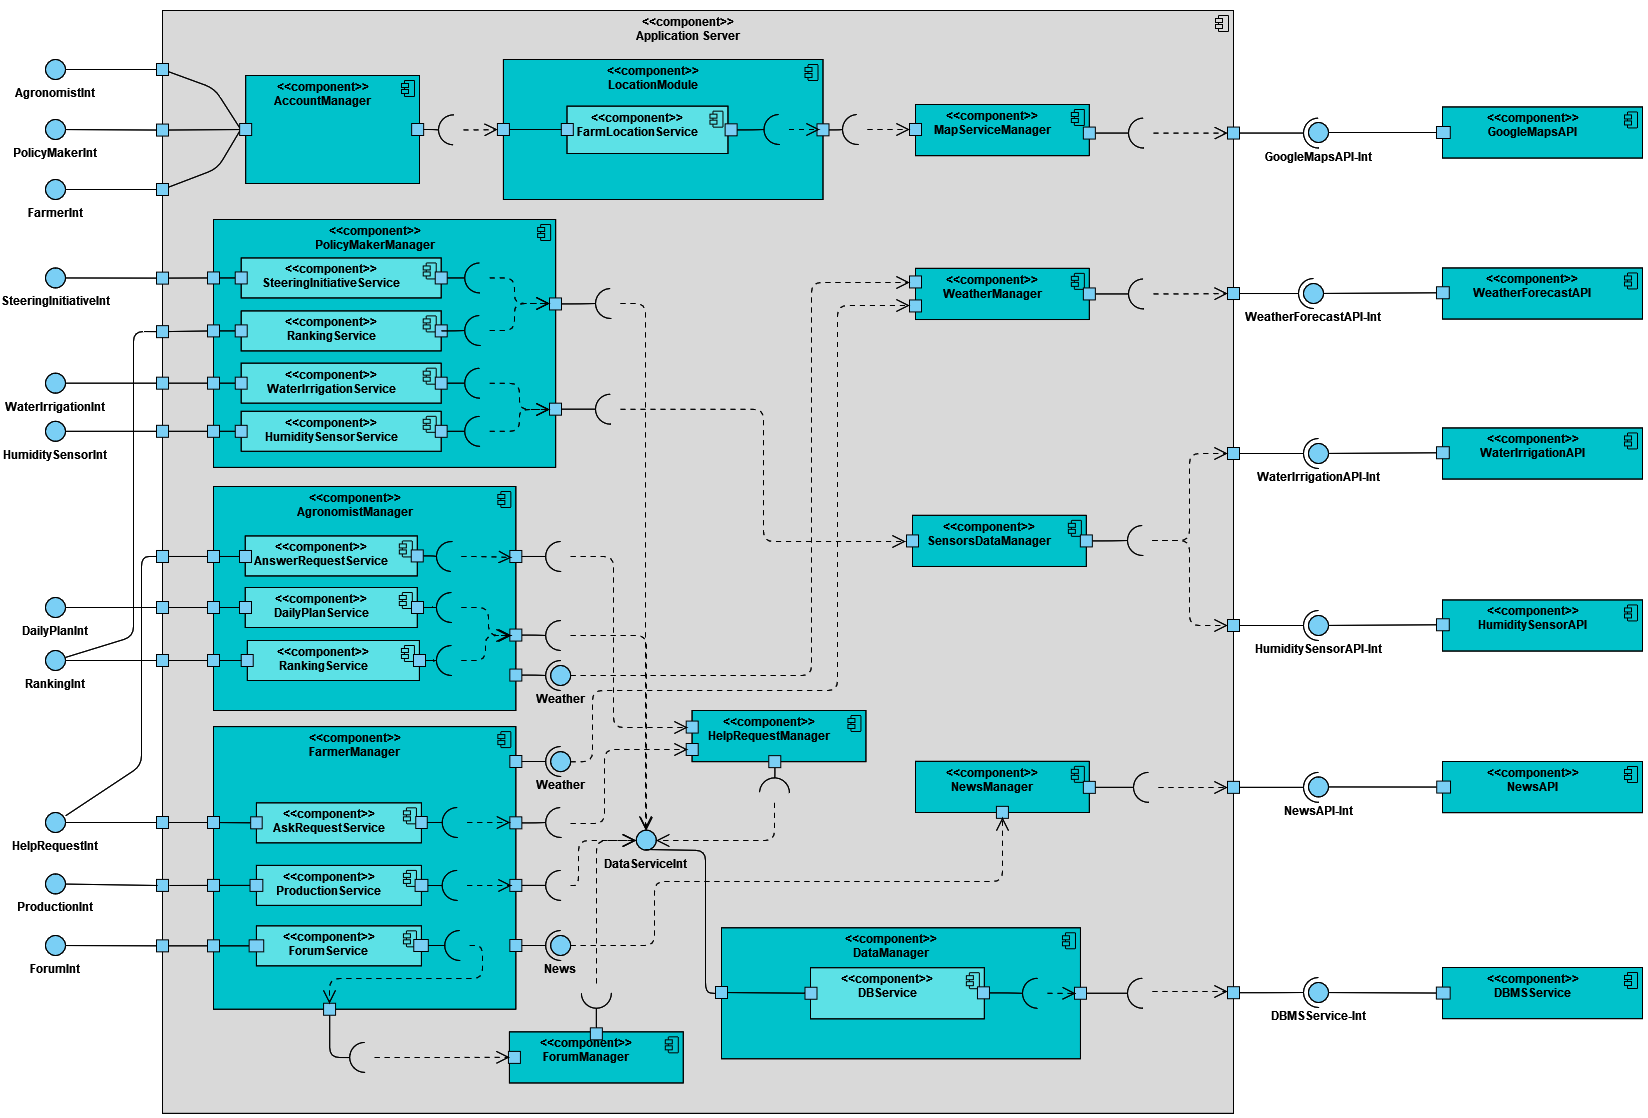
\includegraphics[scale=0.45, center]{assets/application-server-component.png}
        \caption{Application Server Component Diagram}
        \label{fig: application_server_component_view}
    \end{figure}
\end{center}

The following component diagram gives a detailed view of the Application Server, it shows the internal structure and the interaction between the components.
External elements in the diagram are represented in a simplified way.
\begin{itemize}
    \item \textbf{AccountManager}: this component handles all the basic requests made by the client.
    This includes the authentication process that is composed by the log in, the log out and the sign up services. 
    It also includes the edit profile routine invoked by an user editing the personal account.
    Once a user is logged in, all the specific functionalities are provided by the component that manages this type of user.
    Finally it communicates with the \textit{LocationModule} that provides the geolocalization service.
    \item \textbf{LocationModule}: this module provides the interface that allows the geolocalization of the farm based on the GPS and on the address provided by the farmer.
    In order to provide this service, it communicates with the map service manager.
    \item \textbf{MapServiceManager}: this component communicates directly with the external API provided by Google Maps, it provides information regarding the region and allows the user to visualize the map of a specific location.
    Mainly it adapts the data received by the API in a comprehensible way for the other components, it also manages the API requests.
    \item \textbf{PolicyMakerManager}: it manages the policy maker services, these include: steering initiatives, ranking, water irrigation system and humidity sensors.
    The steering initiative service and the ranking service are mapped through an interface to the internal database, on the other side the water irrigation service and the humidity sensor service are considered external services and for this reason are linked to an external database.
    \item \textbf{AgronomistManager}: it manages the agronomist services, these include: answer help requests, daily plan and ranking.
    It includes the weather external interface, it communicates with the weather component in order to provide the weather forecast service to the agronomist.
    The daily plan service and the ranking service are linked to the internal database, instead the answer request service communicates directly with the \textit{HelpRequestManager} component.
    \item \textbf{FarmerManager}: it manages the farmer services, these include: ask a help request, production and forum.
    It includes two external interfaces: the first one communicates with the \textit{WeatherManager} component in order to provide the weather forecast service to the farmer, the other one communicates with the \textit{NewsManager} component.
    In this case, only the production service is linked directly to the internal database, instead the ask request service is linked to the \textit{HelpRequestManager} component, while the forum service exposes an interface to connect to the \textit{ForumManager} component.
    \item \textbf{ForumManager}: this component manages the forum section, in particular it is responsible of the management of all the topics with the related messages between farmers.
    \item \textbf{DataManager}: it provides access to the external interface of the database, it manages queries and interacts with both the internal and the external databases.
    It includes two components: one is responsible of the operations with the external database, the other of the internal database.
    Both these components expose the related interface in order to use the service.
    This component is connected to the \textit{DBMSService} external component, this establishes the connection between the Application Server and the Database Server.
    \item \textbf{HelpRequestManager}: it manages the help requests between farmers and agronomists.
    It communicates with the \textit{FarmerManager} component for the help requests to ask, on the other way it communicates with the \textit{AgronomistManager} component for the ones to answer.
    Finally it provides an interface that communicate with the internal database in order to store the requests.
    \item \textbf{NewsManager}: this component manages the service related to the news, it provides updated suggestions about crops and fertilizers for the farmers.
    To do this it interacts with the external component \textit{NewsService}.
    \item \textbf{WeatherManager}: this component manages the service related to the weather forecast.
    It interacts with the external component \textit{WeatherForecastService} in order to get the weather data.
\end{itemize}

\subsection{Deployment view}

\newpage
\subsection{Runtime view}

Here are represented the runtime view of some relevant uses case of the system through some sequence diagrams. 
In the diagrams, the part regarding the user is omitted because it has been considered superfluous to the understanding of the interaction.
In later diagrams some parts, like the login phase or the come back to home page, were omitted for the above motivations.

\newpage
\textbf{Sign Up}
\begin{center}
    \begin{figure}[H]
        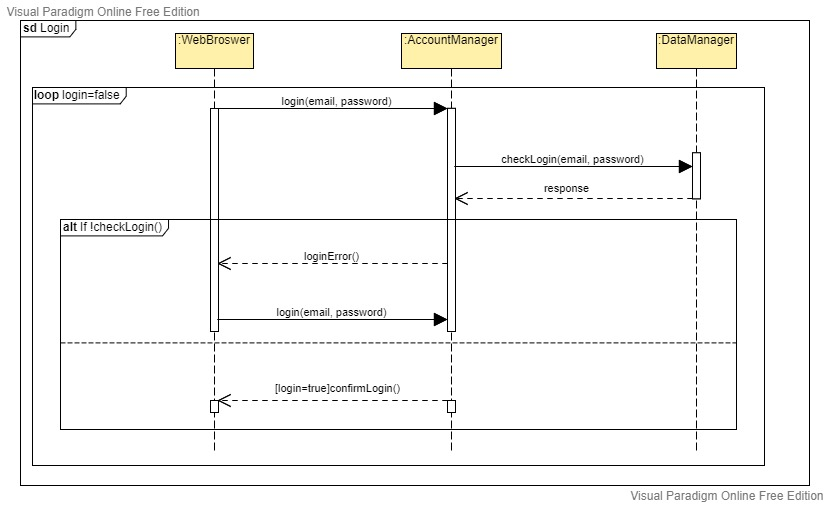
\includegraphics[scale=0.38, center]{assets/SequenceDiagram/SignUp.jpg}
        \caption{Sign Up phase}
        \label{fig:signup}
    \end{figure}
\end{center}
Sign up is pretty standard: user registers himself/herself by inserting first name, last name, email, password, job role and area. If the user is a farmer, he/she chooses also the crop type the farm deals with.
The Location module and Map service are used in this phase in order to ease the users in the selection of their location using the GPS. 
However users can also select manually their location without the use of GPS.

At the end of the process, if every check results succesful, the user is registered into the database by the Data Manager component.

\newpage
\textbf{Log In}
\begin{center}
    \begin{figure}[H]
        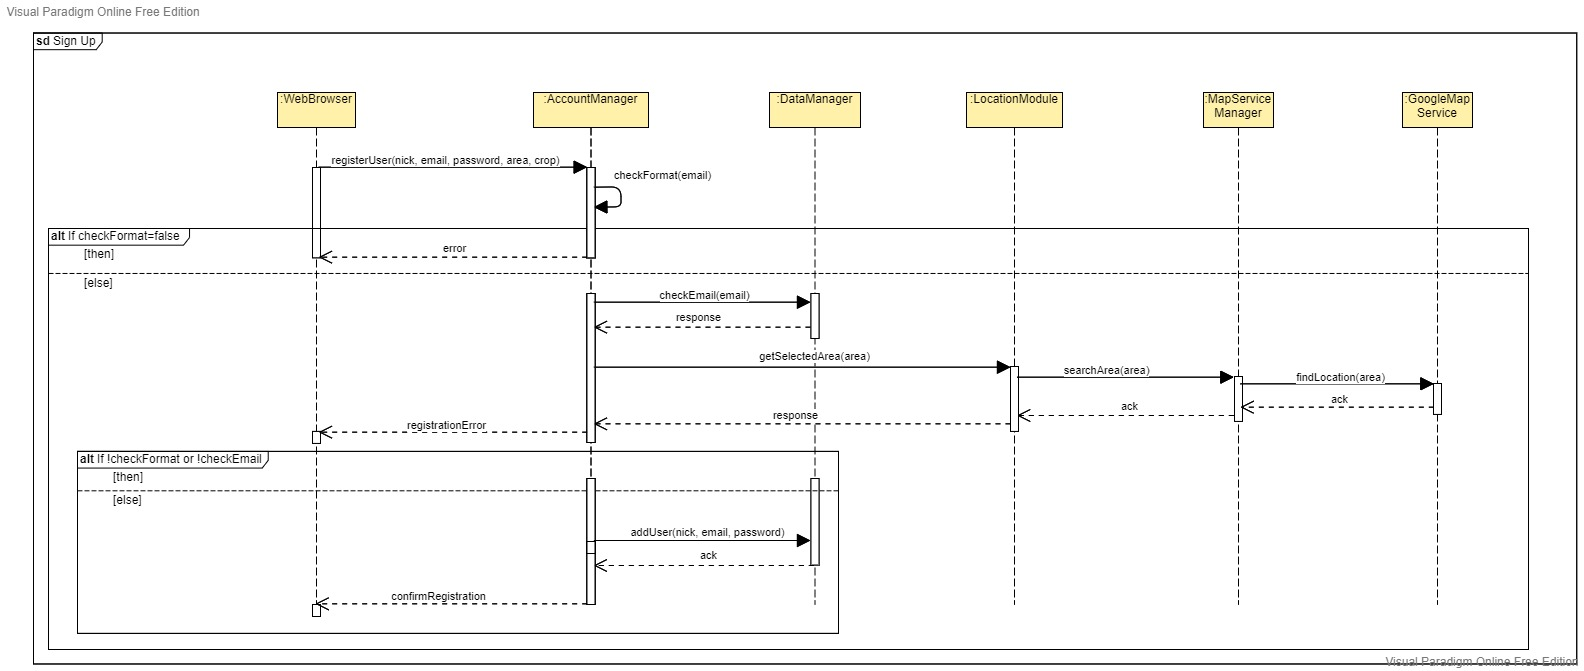
\includegraphics[scale=0.6, center]{assets/SequenceDiagram/Login.jpg}
        \caption{Login Phase}
        \label{fig: login}
    \end{figure}
\end{center}

The Log In phase simply consits in the user action of inserting their email (primary and unique key of the database) and password in the login fields, then the system checks if the pair corresponds to an entry in the database.
In case of success, the user can log in the system and use its functionalities available for that particular type of account chosen during the Sign Up phase.

\newpage
\textbf{View Steering Initiative Reports}
\begin{center}
    \begin{figure}[H]
        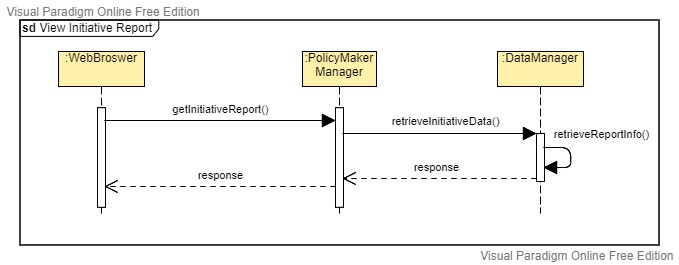
\includegraphics[scale=0.6, center]{assets/SequenceDiagram/Report.jpg}
        \caption{View Initiative reports}
        \label{fig: report}
    \end{figure}
\end{center}
This sequence diagram represents the interactions between components that occur when displaying the steering initiatives (previously stored in the database) to a policy maker user.

\newpage
\textbf{Check Soil Humidity Data}
\begin{center}
    \begin{figure}[H]
        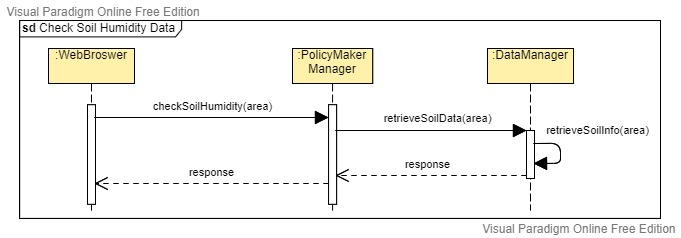
\includegraphics[scale=0.6, center]{assets/SequenceDiagram/Soil.jpg}
        \caption{Check Soil Humidity Sensors Data}
        \label{fig: humidity}
    \end{figure}
\end{center}
This sequence diagram represents the interactions between components that occur when displaying the sensors data regarding soil humidity to a policy maker user.
The business logic running on the Application Server retrieves these data from an external source, furthermore it handles them just temporarely since they are not modified by our system and they're fetched on user demand.   

\newpage
\textbf{Check Water Irrigation Data} 
\begin{center}
    \begin{figure}[H]
        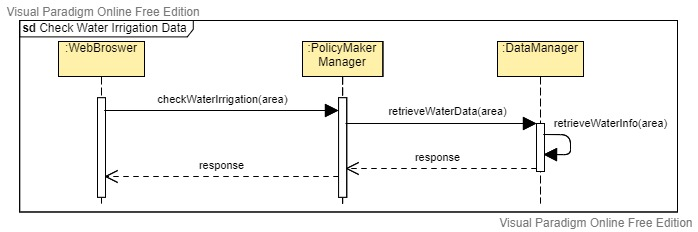
\includegraphics[scale=0.6, center]{assets/SequenceDiagram/Irrigation.jpg}
        \caption{Check Water Irrigation Sensors Data}
        \label{fig: irrigation}
    \end{figure}
\end{center}
This sequence diagram represents the interactions between components that occur when displaying the sensors data regarding the water irrigation to a policy maker user.
The function is the same of the above mentioned case.

\newpage
\textbf{View Farmers Ranking}
\begin{center}
    \begin{figure}[H]
        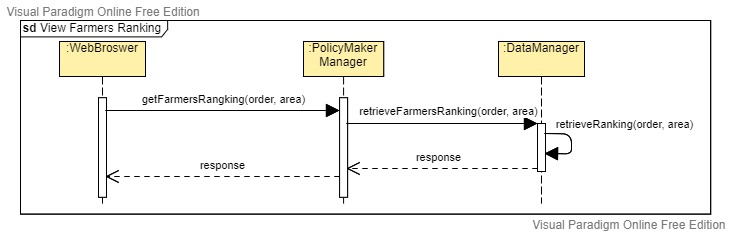
\includegraphics[scale=0.6, center]{assets/SequenceDiagram/Ranking.jpg}
        \caption{View Farmers Ranking}
        \label{fig: ranking}
    \end{figure}
\end{center}
This sequence diagram represents the interactions between components that occur when displaying the farmers ranking to policy maker and agronomist users.
It will be explained better later in the document. %add \ref{}
The function includes an area parameter to specify which area the user wants the rank.
In order to achieve code reusability, this function is invoked by either policy makers or agronomists. 
When a policy maker wants to see the rank the parameter \texttt{area} will be set to \texttt{all} in order to obtain the ranking comprehensive of all Telangana's farmer registered in the app.
Instead, when an agronomist wants to use this functionality, \texttt{area} will be automatically taken to his/her respective responsibility area. Thanks to this, the function becomes more modular.

\newpage
\textbf{View Specific Farmers Informations}
\begin{center}
    \begin{figure}[H]
        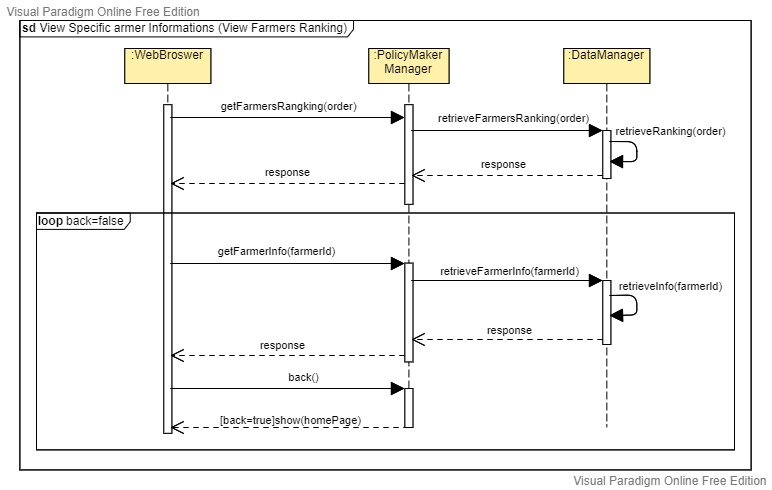
\includegraphics[scale=0.6, center]{assets/SequenceDiagram/SpecificFarmerInfo.jpg}
        \caption{View Specific Farmer Informations}
        \label{fig: specificFarmerInfo}
    \end{figure}
\end{center}
This sequence diagram represents the interactions between components caused by a search for a specific farmer information summary.

\newpage
\textbf{Profile Edit}
\begin{center}
    \begin{figure}[H]
        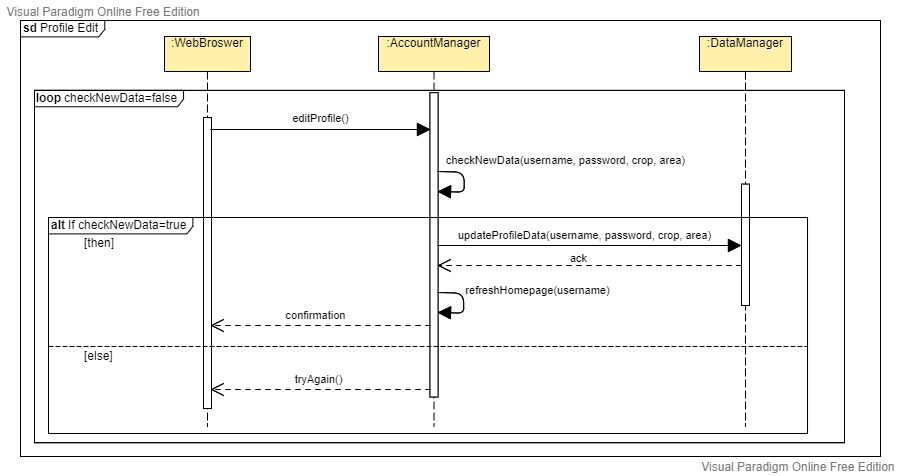
\includegraphics[scale=0.6, center]{assets/SequenceDiagram/ProfileEdit.jpg}
        \caption{Edit Profile}
        \label{fig: profileEdit}
    \end{figure}
\end{center}
This sequence diagram represents the interactions between components that occur when users make changes in the profile settings: edit username, password, area or crop type (if they're farmer users).

\newpage
\textbf{Insert Production Data}
\begin{center}
    \begin{figure}[H]
        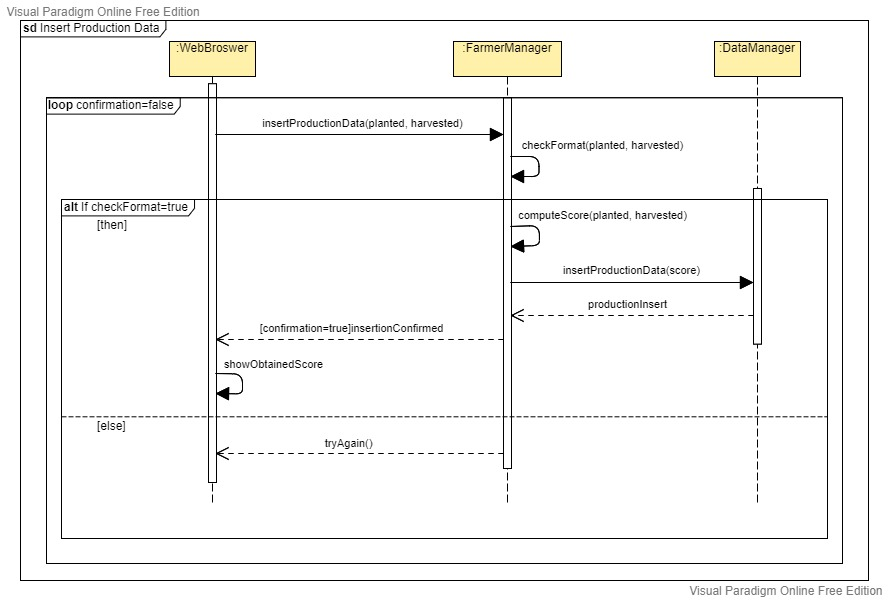
\includegraphics[scale=0.6, center]{assets/SequenceDiagram/InsertProduction.jpg}
        \caption{Insert Production Data}
        \label{fig: production}
    \end{figure}
\end{center}
This sequence diagram represents the interactions between components caused by an insertion of production data from a farmer user.
Each new production entry cause the score associated to the farmer to be calculated again and updated. So the score shall be an attribute of each farmer profile. Since a farmer's rank is directly proportionated to the his/her score, the recomputation can lead to a shifting in the general ranking too.

\newpage
\textbf{Check News}
\begin{center}
    \begin{figure}[H]
        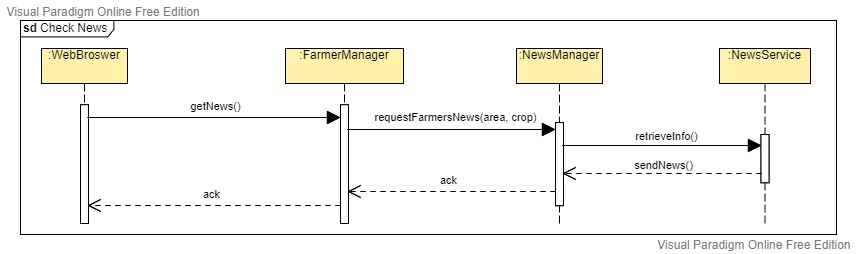
\includegraphics[scale=0.6, center]{assets/SequenceDiagram/CheckNews.jpg}
        \caption{Check News}
        \label{fig: news}
    \end{figure}
\end{center}
This sequence diagram represents the interactions between components that occur when displaying the news regarding farmers' interests to them, such as news concering the same area or crop type of the farmer.
It uses the NewsService component in order to get always up-to-date news and all it's managed by the NewsManager component.

\newpage
\textbf{Forum}
\begin{center}
    \begin{figure}[H]
        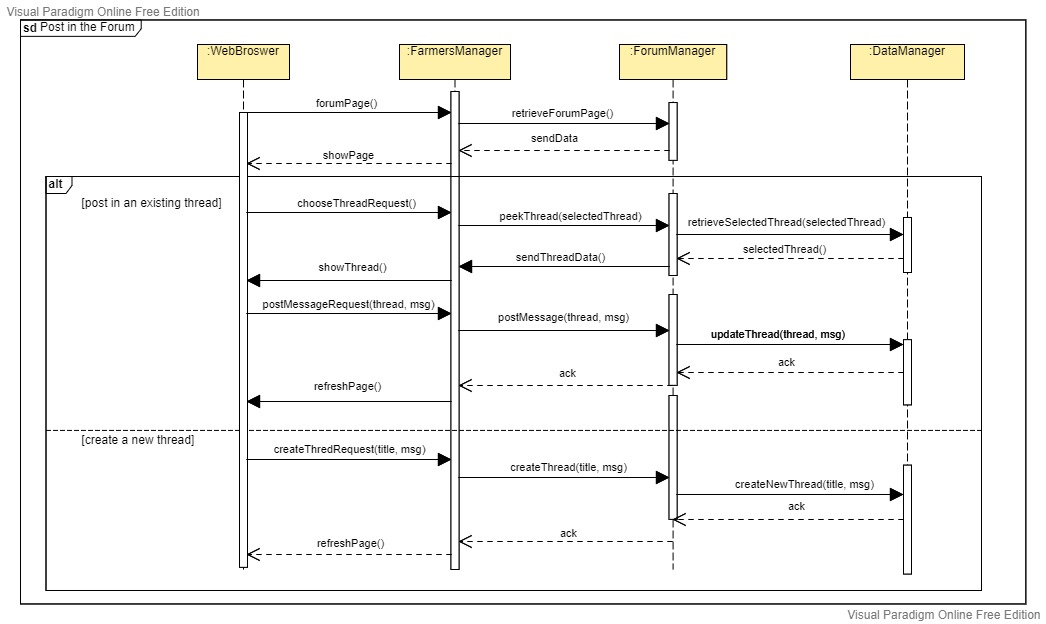
\includegraphics[scale=0.55, center]{assets/SequenceDiagram/Forum.jpg}
        \caption{Interact with Forum}
        \label{fig: forum}
    \end{figure}
\end{center}
This sequence diagram represents the interactions between the components of the forum. 
It is split into two part: the one that allows the user to make a post in an already existing thread and the one that allows the user to create a new thread.

\newpage
\textbf{Check Weathar Forecast}
\begin{center}
    \begin{figure}[H]
        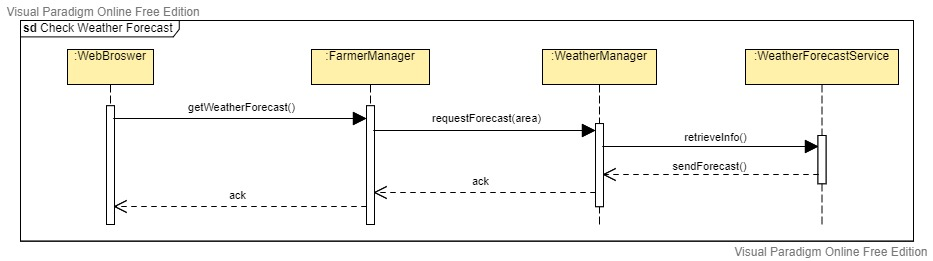
\includegraphics[scale=0.6, center]{assets/SequenceDiagram/Forecast.jpg}
        \caption{Check the Weather Forecasat}
        \label{fig: forecast}
    \end{figure}
\end{center}
This sequence diagram represents the interactions between components that occur when displaying the weather forecast to the users. The weather report is tailored to the user area.
It uses the WeatherForecastService component in order to get always up-to-date forecast and all it's managed by the WeatherManager component.

\newpage
\textbf{Help Request Interaction}
\begin{center}
    \begin{figure}[H]
        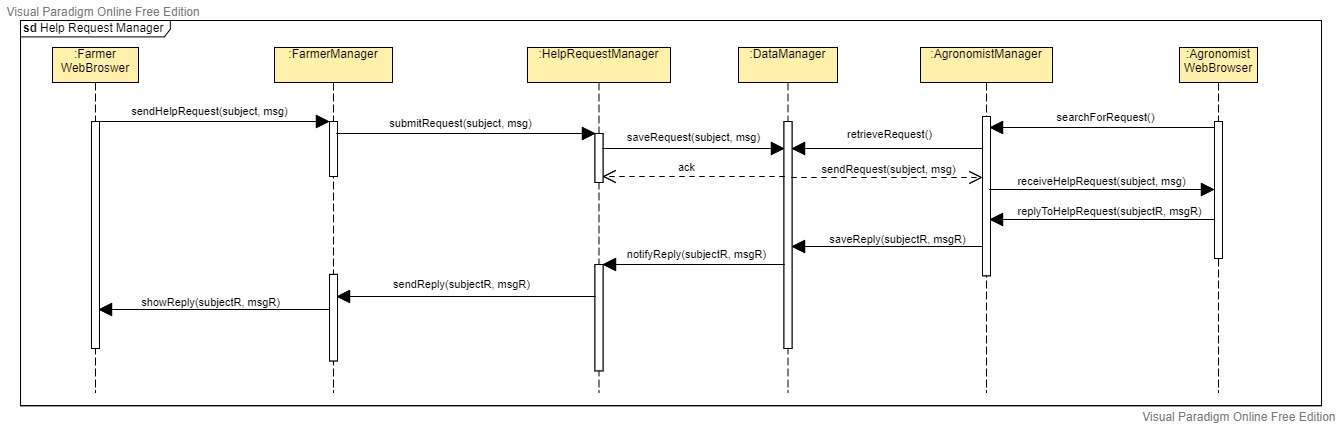
\includegraphics[scale=0.45, center]{assets/SequenceDiagram/HelpRequest.jpg}
        \caption{Help Request Interactions}
        \label{fig: helpRequest}
    \end{figure}
\end{center}
This sequence diagram represents the interactions between the components needed to manage the help requests that the farmers send to the agronomists.
When a farmer sends a help request the system saves it in the database.
When the agronomist is online an automatic script checks if there are some unread messages in the database and sends them to the agronomist.
The agronomist replies to the request and saves it into the database. 
When the farmer is online another automatic script checks if there are some unread replies in the database and displays them to the farmer.
Since the exchange is necessarly asyncronous because of the fact that the receiver of the message might be offline in the moment of the delivery, the messages have to be stored on the database and the unread ones have to be fetched each time the user is back online.   

\newpage
\textbf{Daily Plan Management}
\begin{center}
    \begin{figure}[H]
        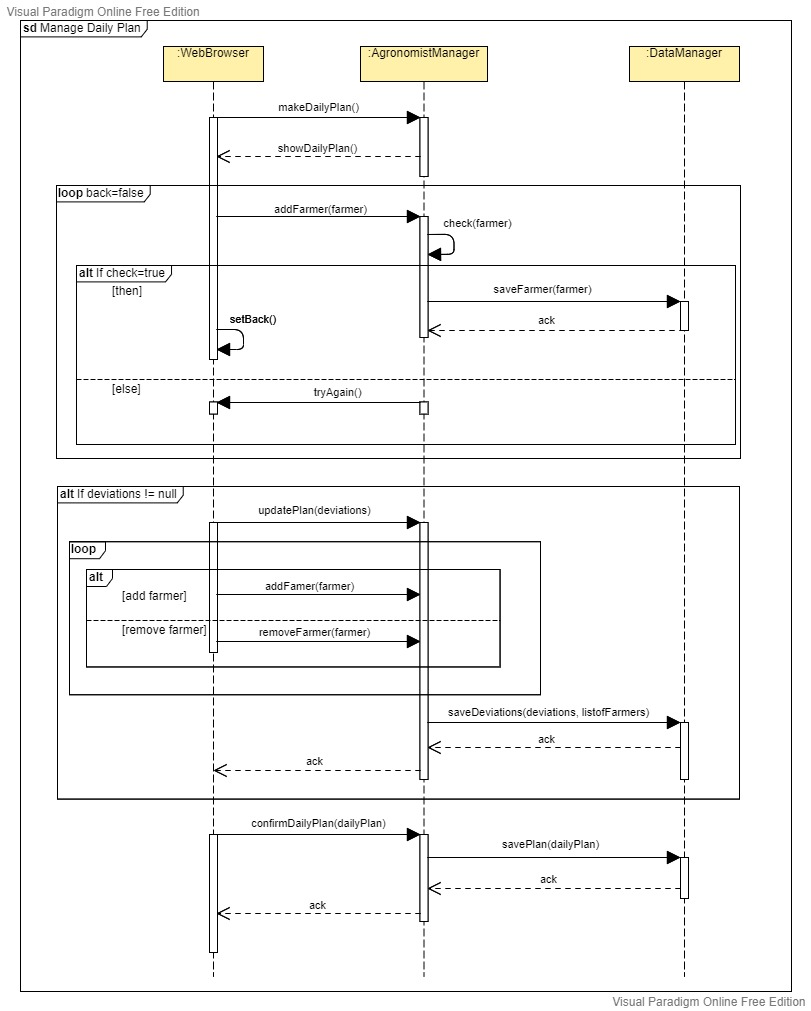
\includegraphics[scale=0.47, center]{assets/SequenceDiagram/DailyPlan.jpg}
        \caption{Daily Plan Interactions}
        \label{fig: dailyPlan}
    \end{figure}
\end{center}
This sequence diagram represents the interactions between components in managing the daily plan.
In the diagram, there are both the creation and the update of the plan.





\subsection{Component interfaces}

\subsection{Selected architectural styles and patterns}

\subsection{Other design decisions}

\section{User Interface Design}


\section{Requirements Traceability}


\section{Implementation, Integration and Test Plan}


\section{Effort Spent}


\section{References}


\end{document}